% Options for packages loaded elsewhere
\PassOptionsToPackage{unicode}{hyperref}
\PassOptionsToPackage{hyphens}{url}
\PassOptionsToPackage{dvipsnames,svgnames*,x11names*}{xcolor}
%
\documentclass[
  8pt,
  ignorenonframetext,
  dvipsnames]{beamer}
\usepackage{pgfpages}
\setbeamertemplate{caption}[numbered]
\setbeamertemplate{caption label separator}{: }
\setbeamercolor{caption name}{fg=normal text.fg}
\beamertemplatenavigationsymbolsempty
% Prevent slide breaks in the middle of a paragraph
\widowpenalties 1 10000
\raggedbottom
\setbeamertemplate{part page}{
  \centering
  \begin{beamercolorbox}[sep=16pt,center]{part title}
    \usebeamerfont{part title}\insertpart\par
  \end{beamercolorbox}
}
\setbeamertemplate{section page}{
  \centering
  \begin{beamercolorbox}[sep=12pt,center]{part title}
    \usebeamerfont{section title}\insertsection\par
  \end{beamercolorbox}
}
\setbeamertemplate{subsection page}{
  \centering
  \begin{beamercolorbox}[sep=8pt,center]{part title}
    \usebeamerfont{subsection title}\insertsubsection\par
  \end{beamercolorbox}
}
\AtBeginPart{
  \frame{\partpage}
}
\AtBeginSection{
  \ifbibliography
  \else
    \frame{\sectionpage}
  \fi
}
\AtBeginSubsection{
  \frame{\subsectionpage}
}
\usepackage{lmodern}
\usepackage{amssymb,amsmath}
\usepackage{ifxetex,ifluatex}
\ifnum 0\ifxetex 1\fi\ifluatex 1\fi=0 % if pdftex
  \usepackage[T1]{fontenc}
  \usepackage[utf8]{inputenc}
  \usepackage{textcomp} % provide euro and other symbols
\else % if luatex or xetex
  \usepackage{unicode-math}
  \defaultfontfeatures{Scale=MatchLowercase}
  \defaultfontfeatures[\rmfamily]{Ligatures=TeX,Scale=1}
\fi
% Use upquote if available, for straight quotes in verbatim environments
\IfFileExists{upquote.sty}{\usepackage{upquote}}{}
\IfFileExists{microtype.sty}{% use microtype if available
  \usepackage[]{microtype}
  \UseMicrotypeSet[protrusion]{basicmath} % disable protrusion for tt fonts
}{}
\makeatletter
\@ifundefined{KOMAClassName}{% if non-KOMA class
  \IfFileExists{parskip.sty}{%
    \usepackage{parskip}
  }{% else
    \setlength{\parindent}{0pt}
    \setlength{\parskip}{6pt plus 2pt minus 1pt}}
}{% if KOMA class
  \KOMAoptions{parskip=half}}
\makeatother
\usepackage{xcolor}
\IfFileExists{xurl.sty}{\usepackage{xurl}}{} % add URL line breaks if available
\IfFileExists{bookmark.sty}{\usepackage{bookmark}}{\usepackage{hyperref}}
\hypersetup{
  pdftitle={Introduction to Multivariate Regression \& Econometrics},
  pdfauthor={Lecture 1},
  colorlinks=true,
  linkcolor=Maroon,
  filecolor=Maroon,
  citecolor=Blue,
  urlcolor=blue,
  pdfcreator={LaTeX via pandoc}}
\urlstyle{same} % disable monospaced font for URLs
\newif\ifbibliography
\usepackage{color}
\usepackage{fancyvrb}
\newcommand{\VerbBar}{|}
\newcommand{\VERB}{\Verb[commandchars=\\\{\}]}
\DefineVerbatimEnvironment{Highlighting}{Verbatim}{commandchars=\\\{\}}
% Add ',fontsize=\small' for more characters per line
\usepackage{framed}
\definecolor{shadecolor}{RGB}{248,248,248}
\newenvironment{Shaded}{\begin{snugshade}}{\end{snugshade}}
\newcommand{\AlertTok}[1]{\textcolor[rgb]{0.94,0.16,0.16}{#1}}
\newcommand{\AnnotationTok}[1]{\textcolor[rgb]{0.56,0.35,0.01}{\textbf{\textit{#1}}}}
\newcommand{\AttributeTok}[1]{\textcolor[rgb]{0.77,0.63,0.00}{#1}}
\newcommand{\BaseNTok}[1]{\textcolor[rgb]{0.00,0.00,0.81}{#1}}
\newcommand{\BuiltInTok}[1]{#1}
\newcommand{\CharTok}[1]{\textcolor[rgb]{0.31,0.60,0.02}{#1}}
\newcommand{\CommentTok}[1]{\textcolor[rgb]{0.56,0.35,0.01}{\textit{#1}}}
\newcommand{\CommentVarTok}[1]{\textcolor[rgb]{0.56,0.35,0.01}{\textbf{\textit{#1}}}}
\newcommand{\ConstantTok}[1]{\textcolor[rgb]{0.00,0.00,0.00}{#1}}
\newcommand{\ControlFlowTok}[1]{\textcolor[rgb]{0.13,0.29,0.53}{\textbf{#1}}}
\newcommand{\DataTypeTok}[1]{\textcolor[rgb]{0.13,0.29,0.53}{#1}}
\newcommand{\DecValTok}[1]{\textcolor[rgb]{0.00,0.00,0.81}{#1}}
\newcommand{\DocumentationTok}[1]{\textcolor[rgb]{0.56,0.35,0.01}{\textbf{\textit{#1}}}}
\newcommand{\ErrorTok}[1]{\textcolor[rgb]{0.64,0.00,0.00}{\textbf{#1}}}
\newcommand{\ExtensionTok}[1]{#1}
\newcommand{\FloatTok}[1]{\textcolor[rgb]{0.00,0.00,0.81}{#1}}
\newcommand{\FunctionTok}[1]{\textcolor[rgb]{0.00,0.00,0.00}{#1}}
\newcommand{\ImportTok}[1]{#1}
\newcommand{\InformationTok}[1]{\textcolor[rgb]{0.56,0.35,0.01}{\textbf{\textit{#1}}}}
\newcommand{\KeywordTok}[1]{\textcolor[rgb]{0.13,0.29,0.53}{\textbf{#1}}}
\newcommand{\NormalTok}[1]{#1}
\newcommand{\OperatorTok}[1]{\textcolor[rgb]{0.81,0.36,0.00}{\textbf{#1}}}
\newcommand{\OtherTok}[1]{\textcolor[rgb]{0.56,0.35,0.01}{#1}}
\newcommand{\PreprocessorTok}[1]{\textcolor[rgb]{0.56,0.35,0.01}{\textit{#1}}}
\newcommand{\RegionMarkerTok}[1]{#1}
\newcommand{\SpecialCharTok}[1]{\textcolor[rgb]{0.00,0.00,0.00}{#1}}
\newcommand{\SpecialStringTok}[1]{\textcolor[rgb]{0.31,0.60,0.02}{#1}}
\newcommand{\StringTok}[1]{\textcolor[rgb]{0.31,0.60,0.02}{#1}}
\newcommand{\VariableTok}[1]{\textcolor[rgb]{0.00,0.00,0.00}{#1}}
\newcommand{\VerbatimStringTok}[1]{\textcolor[rgb]{0.31,0.60,0.02}{#1}}
\newcommand{\WarningTok}[1]{\textcolor[rgb]{0.56,0.35,0.01}{\textbf{\textit{#1}}}}
\usepackage{longtable,booktabs}
\usepackage{caption}
% Make caption package work with longtable
\makeatletter
\def\fnum@table{\tablename~\thetable}
\makeatother
\usepackage{graphicx,grffile}
\makeatletter
\def\maxwidth{\ifdim\Gin@nat@width>\linewidth\linewidth\else\Gin@nat@width\fi}
\def\maxheight{\ifdim\Gin@nat@height>\textheight\textheight\else\Gin@nat@height\fi}
\makeatother
% Scale images if necessary, so that they will not overflow the page
% margins by default, and it is still possible to overwrite the defaults
% using explicit options in \includegraphics[width, height, ...]{}
\setkeys{Gin}{width=\maxwidth,height=\maxheight,keepaspectratio}
% Set default figure placement to htbp
\makeatletter
\def\fps@figure{htbp}
\makeatother
\setlength{\emergencystretch}{3em} % prevent overfull lines
\providecommand{\tightlist}{%
  \setlength{\itemsep}{0pt}\setlength{\parskip}{0pt}}
\setcounter{secnumdepth}{-\maxdimen} % remove section numbering

%packages
\usepackage{graphicx}
\usepackage{rotating}
\usepackage{hyperref}

\usepackage{tikz} % used for text highlighting, amongst others
\usepackage{comment}

%title slide stuff
%\institute{Department of Education}
%\title{Managing and Manipulating Data Using R}

%
\setbeamertemplate{navigation symbols}{} % get rid of navigation icons:
\setbeamertemplate{footline}[page number]

%\setbeamertemplate{frametitle}{\thesection \hspace{0.2cm} \insertframetitle}
\setbeamertemplate{section in toc}[sections numbered]
%\setbeamertemplate{subsection in toc}[subsections numbered]
\setbeamertemplate{subsection in toc}{%
  \leavevmode\leftskip=3.2em\color{gray}\rlap{\hskip-2em\inserttocsectionnumber.\inserttocsubsectionnumber}\inserttocsubsection\par
}

%define colors
%\definecolor{uva_orange}{RGB}{216,141,42} % UVa orange (Rotunda orange)
\definecolor{mygray}{rgb}{0.95, 0.95, 0.95} % for highlighted text
	% grey is equal parts red, green, blue. higher values >> lighter grey
	%\definecolor{lightgraybo}{rgb}{0.83, 0.83, 0.83}

% new commands

%highlight text with very light grey
\newcommand*{\hlg}[1]{%
	\tikz[baseline=(X.base)] \node[rectangle, fill=mygray] (X) {#1};%
}
%, inner sep=0.3mm
%highlight text with very light grey and use font associated with code
\newcommand*{\hlgc}[1]{\texttt{\hlg{#1}}}

%modifying back ticks to add grey background
\let\OldTexttt\texttt
\renewcommand{\texttt}[1]{\OldTexttt{\hlg{#1}}}


\begin{comment}

% Font
\usepackage[defaultfam,light,tabular,lining]{montserrat}
\usepackage[T1]{fontenc}
\renewcommand*\oldstylenums[1]{{\fontfamily{Montserrat-TOsF}\selectfont #1}}

% Change color of boldface text to darkgray
\renewcommand{\textbf}[1]{{\color{darkgray}\bfseries\fontfamily{Montserrat-TOsF}#1}}

% Bullet points
\setbeamertemplate{itemize item}{\color{BlueViolet}$\circ$}
\setbeamertemplate{itemize subitem}{\color{BrickRed}$\triangleright$}
\setbeamertemplate{itemize subsubitem}{$-$}

% Reduce space before lists
%\addtobeamertemplate{itemize/enumerate body begin}{}{\vspace*{-8pt}}

\let\olditem\item
\renewcommand{\item}{%
  \olditem\vspace{4pt}
}

% decreasing space before and after level-2 bullet block
%\addtobeamertemplate{itemize/enumerate subbody begin}{}{\vspace*{-3pt}}
%\addtobeamertemplate{itemize/enumerate subbody end}{}{\vspace*{-3pt}}

% decreasing space before and after level-3 bullet block
%\addtobeamertemplate{itemize/enumerate subsubbody begin}{}{\vspace*{-2pt}}
%\addtobeamertemplate{itemize/enumerate subsubbody end}{}{\vspace*{-2pt}}

%Section numbering
\setbeamertemplate{section page}{%
    \begingroup
        \begin{beamercolorbox}[sep=10pt,center,rounded=true,shadow=true]{section title}
        \usebeamerfont{section title}\thesection~\insertsection\par
        \end{beamercolorbox}
    \endgroup
}

\setbeamertemplate{subsection page}{%
    \begingroup
        \begin{beamercolorbox}[sep=6pt,center,rounded=true,shadow=true]{subsection title}
        \usebeamerfont{subsection title}\thesection.\thesubsection~\insertsubsection\par
        \end{beamercolorbox}
    \endgroup
}

\end{comment}

\title{Introduction to Multivariate Regression \& Econometrics}
\subtitle{HED 612}
\author{Lecture 1}
\date{}

\begin{document}
\frame{\titlepage}

\begin{frame}
  \tableofcontents[hideallsubsections]
\end{frame}
\hypertarget{student-introductions}{%
\section{Student Introductions}\label{student-introductions}}

\begin{frame}{Student introductions}
\protect\hypertarget{student-introductions-1}{}

\begin{enumerate}
\tightlist
\item
  Preferred name
\item
  Preferred pronouns
\item
  Academic program (and how far along)
\item
  GA, RA, TA, and/or job?
\item
  Why are you interested in this course?
\end{enumerate}

\end{frame}

\hypertarget{about-your-instructor}{%
\section{About your instructor}\label{about-your-instructor}}

\begin{frame}{Karina Salazar, instructor}
\protect\hypertarget{karina-salazar-instructor}{}

My start in statistical analysis

\begin{itemize}
\tightlist
\item
  Began taking quantitative methods courses as a Master's student

  \begin{itemize}
  \tightlist
  \item
    Material did not come easy to me! I took intro course twice!
  \item
    Took statistics courses in sociology
  \item
    Causal inference courses at The University of Michigan
  \end{itemize}
\end{itemize}

\medskip

\begin{itemize}
\tightlist
\item
  Developed strong data skills

  \begin{itemize}
  \tightlist
  \item
    Getting data ready for analysis is often very time and labor
    intensive!
  \item
    Learned data management skills in SPSS and Stata
  \item
    Learned data science skills in Python and R
  \end{itemize}
\end{itemize}

\medskip

\begin{itemize}
\tightlist
\item
  Applied what I was learning in class.

  \begin{itemize}
  \tightlist
  \item
    Worked in assessment and institutional research offices; evaluated
    retention programs
  \item
    Research assistantship in sociology; worked with national datasets
    (IPEDS, Survey of Earned Doctorates, Higher Education R\&D Survey)
  \end{itemize}
\end{itemize}

\medskip

\begin{itemize}
\tightlist
\item
  Sought out teaching opportunities.

  \begin{itemize}
  \tightlist
  \item
    TA for HED regression and data management courses
  \item
    Delivered practioner-based workshops
  \end{itemize}
\end{itemize}

\end{frame}

\begin{frame}{Enrollment Management Research Program}
\protect\hypertarget{enrollment-management-research-program}{}

\begin{itemize}
\tightlist
\item
  Grew tired of mainstream access inequality policy discourse\ldots{}

  \begin{itemize}
  \tightlist
  \item
    Onus on students, families, and K-12 schools
  \item
    Enrollments can only tell us so much
  \end{itemize}
\end{itemize}

\medskip

\begin{itemize}
\tightlist
\item
  Do the enrollment management policies and practices of public
  universities undermine access for underserved student populations?

  \begin{itemize}
  \tightlist
  \item
    Universities say they care about low-income students, Students of
    Color
  \item
    But who do they actually recruit? Use data science to collect
    recruiting events!
  \end{itemize}
\end{itemize}

\medskip

\begin{itemize}
\tightlist
\item
  Policy implications

  \begin{itemize}
  \tightlist
  \item
    Too many policy decisions for increasing access attempt to ``fix''
    student behavior
  \item
    Assumption: doubling low-income, Students of Color applying to a
    university will double their enrollment
  \end{itemize}
\end{itemize}

Examples:

\begin{itemize}
\tightlist
\item
  \href{https://emraresearch.org/}{The off-campus recruiting project}
\item
  \href{https://ksalazar3.github.io/defense/\#/title}{Dissertation
  Defense}
\end{itemize}

\end{frame}

\hypertarget{what-is-econometrics}{%
\section{What is Econometrics?}\label{what-is-econometrics}}

\begin{frame}{Econometrics (also ``Program Evaluation'', Causal
Inference)}
\protect\hypertarget{econometrics-also-program-evaluation-causal-inference}{}

\textbf{Econometrics} is the main methodological strategy used to assess
the impact of programs, policies, and interventions.

\medskip

The goal of econometrics is to determine the \textbf{causal effect} of
the ``program, policy, or treatment'' (\emph{the independent variable of
interest}) on some educational outcome (\emph{the dependent variable})
by inferring what would have happened in the absence of the ``program,
policy, or treatment'' (\emph{the counterfactual}).

\begin{itemize}
\tightlist
\item
  Do smaller classes improve learning?
\item
  Does offering students financial incentives increase college
  completion?
\item
  Is online instruction as effective as in-class instruction?
\end{itemize}

\medskip

Causal relationships vs.~descriptive statistics

\begin{itemize}
\tightlist
\item
  We often infer causality from correlation
\item
  Ice cream consumption causes drownings vs drownings rise when ice
  cream consumption increases
\item
  Smaller classes cause more learning vs.~students in smaller classes
  have higher test scores
\end{itemize}

\end{frame}

\begin{frame}{Example}
\protect\hypertarget{example}{}

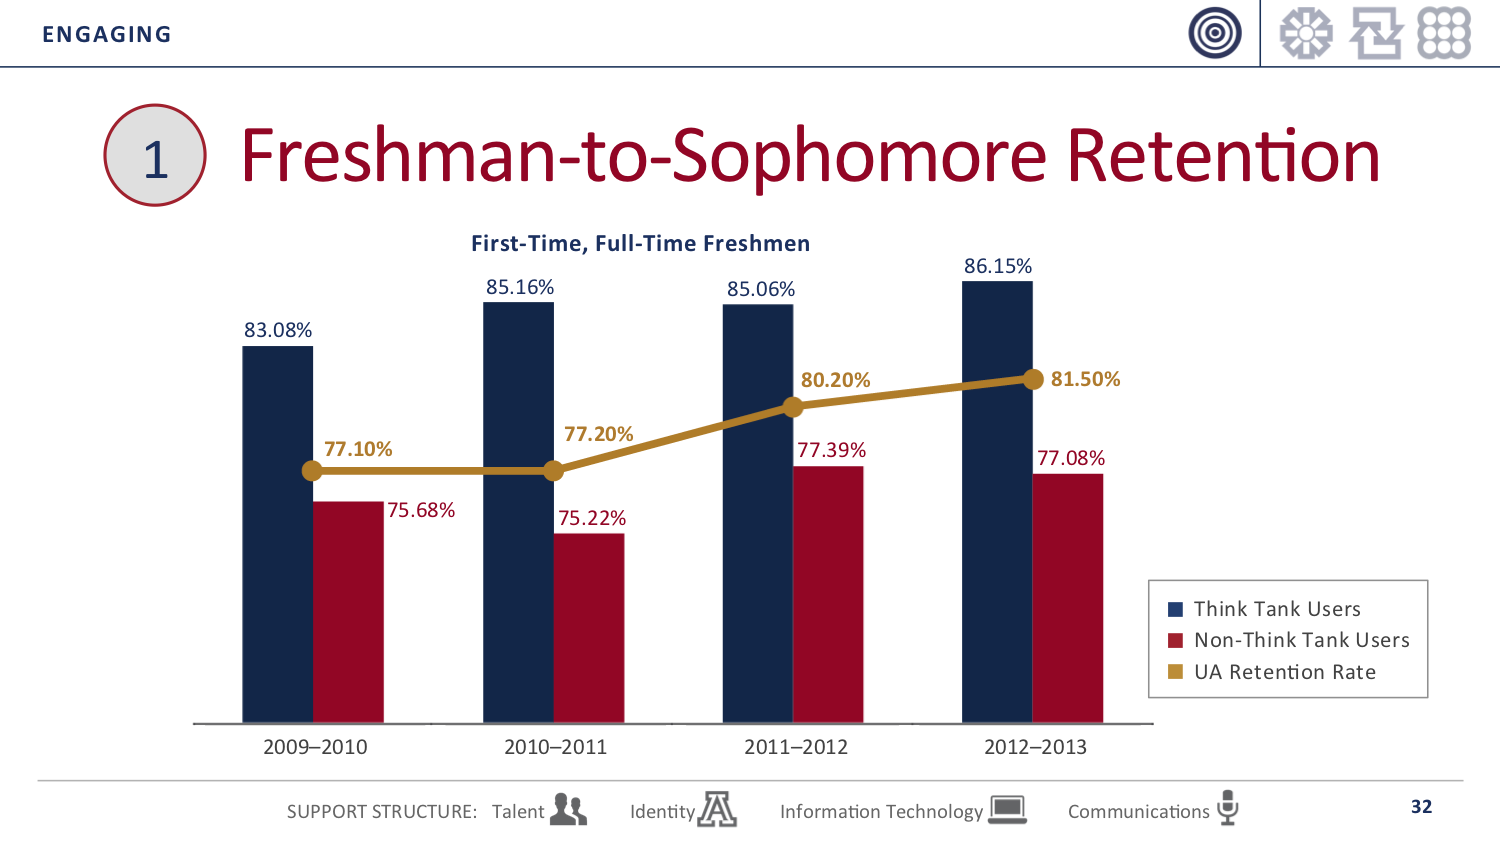
\includegraphics{abor.png}

\end{frame}

\begin{frame}{Econometrics \& Regression}
\protect\hypertarget{econometrics-regression}{}

\textbf{Regression is used to answer both descriptive and causal
questions}

\begin{itemize}
\tightlist
\item
  One is not better than the other, they're just different types of
  research questions!
\item
  You can use the same skills to answer both types of ?s via regression
\end{itemize}

\medskip

\textbf{Why learn regression from an econometrics lens?}

\emph{If you decide to pursue econometrics research}:

\begin{itemize}
\tightlist
\item
  Using regression to overcome \emph{selection bias} in \emph{the
  independent variable of interest} is the first ``tool'' in a
  methodologist's causal inference toolkit.
\item
  Provides the foundation for more rigorous tools

  \begin{itemize}
  \tightlist
  \item
    e.g., Difference-in-Difference, Propensity Score Matching,
    Regression Discontinuity
  \end{itemize}
\end{itemize}

\medskip

\emph{If you decide not to pursue econometrics research}:

\begin{itemize}
\tightlist
\item
  It's easier to learn the fundamentals of regression by focusing on
  \textbf{one} relationship
\item
  Forces you to be thoughtful and intentional about what variables you
  include in regression models even when you're focusing on descriptive
  relationships

  \begin{itemize}
  \tightlist
  \item
    Avoid the ``throwing everything but the kitchen sink'' approach to
    regression modeling
  \end{itemize}
\end{itemize}

\end{frame}

\hypertarget{course-logistics}{%
\section{Course logistics}\label{course-logistics}}

\begin{frame}{Course logistics}
\protect\hypertarget{course-logistics-1}{}

\begin{itemize}
\tightlist
\item
  follow the syllabus
\end{itemize}

\end{frame}

\hypertarget{minute-break}{%
\section{10 MINUTE BREAK}\label{minute-break}}

\hypertarget{what-is-r}{%
\section{What is R}\label{what-is-r}}

\begin{frame}{What is R}
\protect\hypertarget{what-is-r-1}{}

According to the Inter-university consortium for political and social
research
\href{https://www.icpsr.umich.edu/icpsrweb/content/shared/ICPSR/faqs/what-is-r.html}{(ICPSR)}:

\begin{quote}
R is ``an alternative to traditional statistical packages such as SPSS,
SAS, and Stata such that it is an extensible, open-source language and
computing environment for Windows, Macintosh, UNIX, and Linux platforms.
Such software allows for the user to freely distribute, study, change,
and improve the software under the
\href{https://www.gnu.org/home.en.html}{Free Software Foundation's GNU
General Public License}.''
\end{quote}

\begin{itemize}
\tightlist
\item
  For more info visit
  \href{https://www.r-project.org/about.html}{R-project.org}
\end{itemize}

\end{frame}

\begin{frame}[fragile]{Base R vs.~R packages}
\protect\hypertarget{base-r-vs.-r-packages}{}

There are ``default'' packages that come with
\href{https://stat.ethz.ch/R-manual/R-devel/library/base/html/00Index.html}{R}.
Some of these include:

\begin{itemize}
\tightlist
\item
  \texttt{as.character}~\\
\item
  \texttt{print}~\\
\item
  \texttt{setwd}
\end{itemize}

And there are \href{http://r-pkgs.had.co.nz/intro.html}{R packages}
developed and shared by others. Some R packages include:

\begin{itemize}
\tightlist
\item
  \texttt{tidyverse}~\\
\item
  \texttt{stargazer}~\\
\item
  \texttt{equiomatic}
\end{itemize}

more about these in later weeks\ldots{}

\end{frame}

\begin{frame}{RStudio}
\protect\hypertarget{rstudio}{}

``\href{https://www.rstudio.com/products/rstudio/features/}{RStudio} is
an integrated development environment (IDE) for R. It includes a
console, syntax-highlighting editor that supports direct code execution,
as well as tools for plotting, history, debugging and workspace
management.''

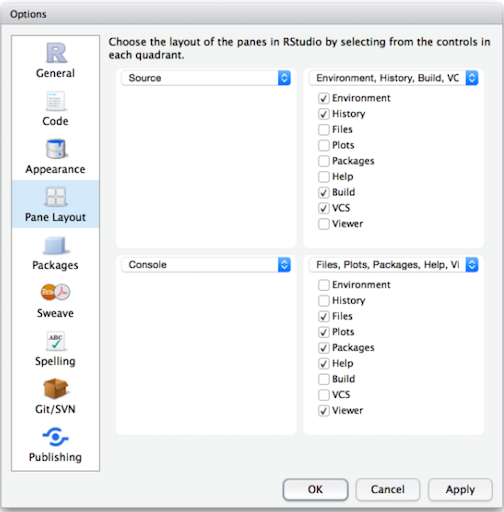
\includegraphics{pane_layout.png}

\end{frame}

\begin{frame}{R Markdown}
\protect\hypertarget{r-markdown}{}

\href{https://rmarkdown.rstudio.com/}{R Markdown} produces dynamic
output formats in html, pdf, MS Word, dashboards, Beamer presentations,
etc.

\end{frame}

\begin{frame}{Why R? Capabilities of R}
\protect\hypertarget{why-r-capabilities-of-r}{}

\begin{itemize}
\tightlist
\item
  \href{http://r-statistics.co/Linear-Regression.html}{Modeling}
\item
  \href{https://ggplot2.tidyverse.org/}{Graphs}
\item
  \href{https://bookdown.org/yihui/rmarkdown/presentations.html}{Presentation}
\item
  \href{https://bookdown.org/yihui/rmarkdown/websites.html}{Websites}
\item
  \href{https://bookdown.org/yihui/rmarkdown/journals.html}{Journals}
\item
  \href{https://rstudio.github.io/learnr/}{Interactive tutorials}
\item
  \href{http://shiny.rstudio.com/}{Web apps}
\item
  \href{https://rmarkdown.rstudio.com/flexdashboard/}{Dashbaords}
\item
  \href{https://bookdown.org/}{Books}\\
\item
  \href{https://www.analyticsvidhya.com/blog/2017/03/beginners-guide-on-web-scraping-in-r-using-rvest-with-hands-on-knowledge/}{Web
  scraping}
\item
  \href{http://pierreroudier.github.io/teaching/20170626-Pedometrics/20170626-soil-data.html}{Maps}
\end{itemize}

For more info \href{https://bookdown.org/yihui/rmarkdown/}{visit}

\end{frame}

\begin{frame}[fragile]{Modeling}
\protect\hypertarget{modeling}{}

Run just about any modeling technique! This course will focus on linear
regression\ldots{}

\medskip

\textbf{Population Regression Model:}

\begin{itemize}
\tightlist
\item
  \(Y_{i} = \beta_{0} + \beta_{1}X_{i} + u_{1}\)
\end{itemize}

\textbf{OLS Prediction Line:}

\begin{itemize}
\tightlist
\item
  \(\hat{Y_{i}} = \hat{\beta_{0}} + \hat{\beta_{1}}X_{i}\)
\end{itemize}

\textbf{What is the effect of engine size (cylinder count) on mpg?}

\begin{itemize}
\tightlist
\item
  \(\hat{\text{mpg}} = \hat{\beta_{0}} + \hat{\beta_{1}}(\text{cyl})\)
\end{itemize}

\medskip

\begin{Shaded}
\begin{Highlighting}[]
\CommentTok{#remotes::install_github("datalorax/equatiomatic")}
\KeywordTok{library}\NormalTok{(equatiomatic)}
\NormalTok{mod1 <-}\StringTok{ }\KeywordTok{lm}\NormalTok{(mpg }\OperatorTok{~}\StringTok{ }\NormalTok{cyl, mtcars)}
\end{Highlighting}
\end{Shaded}

\begin{Shaded}
\begin{Highlighting}[]
\KeywordTok{extract_eq}\NormalTok{(mod1, }\DataTypeTok{use_coefs =} \OtherTok{TRUE}\NormalTok{)}
\end{Highlighting}
\end{Shaded}

\[
\operatorname{mpg} = 37.88 - 2.88(\operatorname{cyl}) + \epsilon
\]

\end{frame}

\begin{frame}[fragile]{Graphs}
\protect\hypertarget{graphs}{}

\begin{itemize}
\tightlist
\item
  Create graphs with \href{https://ggplot2.tidyverse.org/}{ggplot2}
  package
\end{itemize}

\begin{verbatim}
#> `geom_smooth()` using formula 'y ~ x'
\end{verbatim}

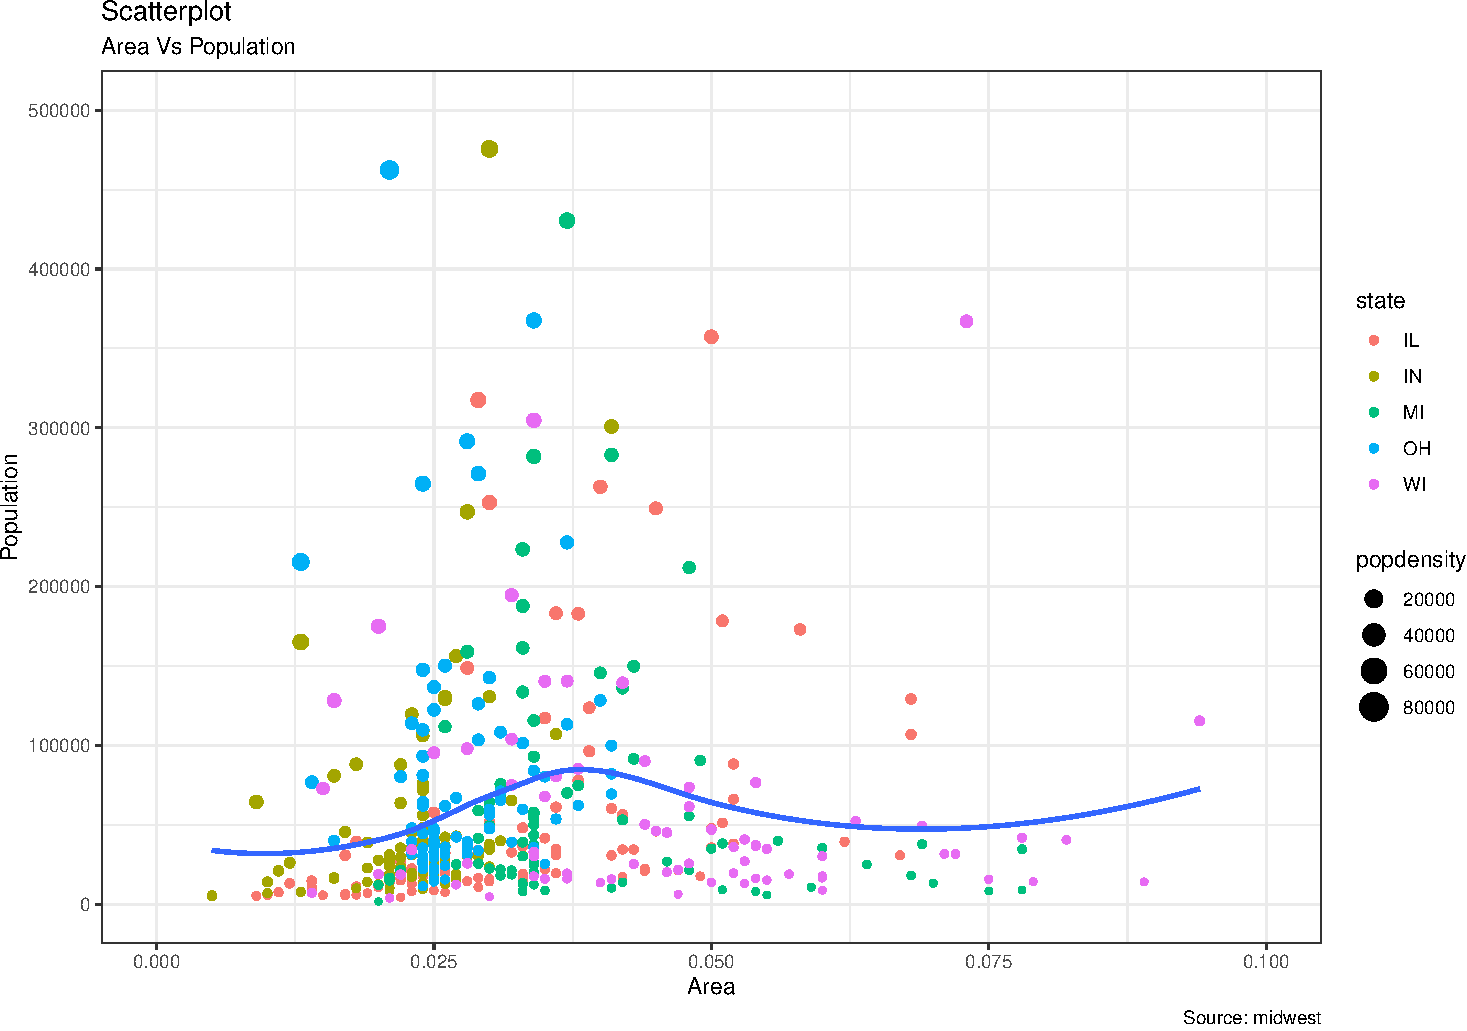
\includegraphics{lecture1_files/figure-beamer/unnamed-chunk-4-1.pdf}

\end{frame}

\begin{frame}{Journal articles}
\protect\hypertarget{journal-articles}{}

\begin{itemize}
\tightlist
\item
  Journal articles with
  \href{https://github.com/rstudio/rticles}{rticles} package
  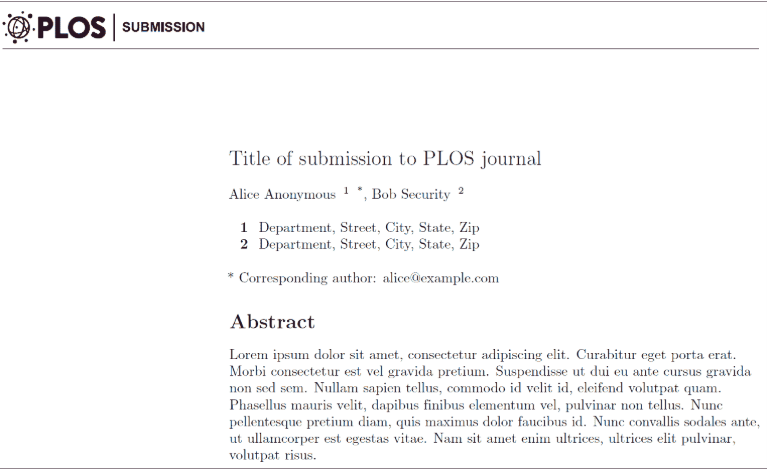
\includegraphics{rticles.png}
\end{itemize}

\end{frame}

\begin{frame}{Interactive web apps}
\protect\hypertarget{interactive-web-apps}{}

\begin{itemize}
\tightlist
\item
  Interactive web apps with \href{http://shiny.rstudio.com/}{shiny}
  package 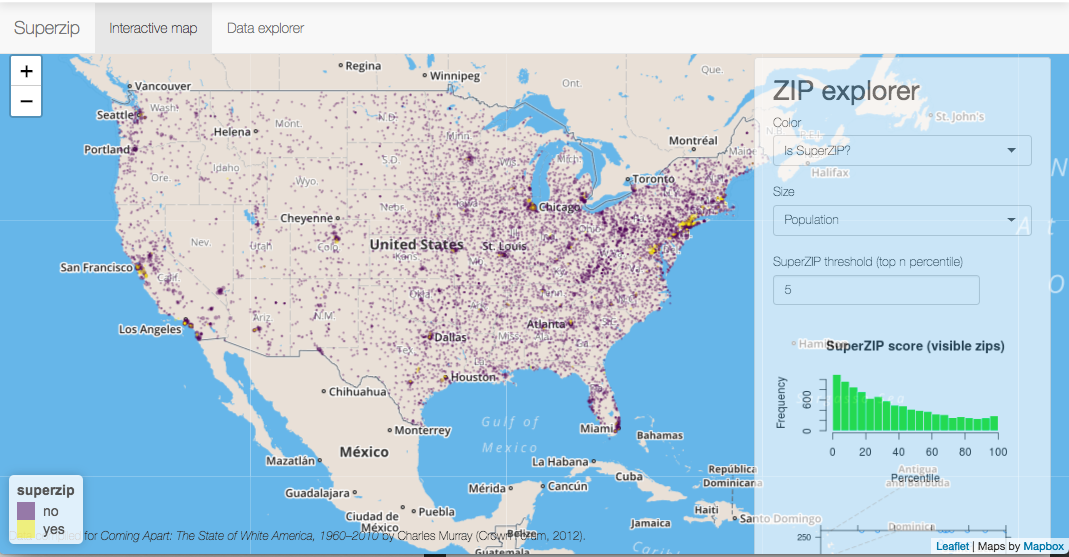
\includegraphics{shiny.png}
\end{itemize}

\end{frame}

\begin{frame}{Mapping}
\protect\hypertarget{mapping}{}

\begin{itemize}
\tightlist
\item
  Mapping with \href{http://strimas.com/r/tidy-sf/}{sf} package \&
  ggplot 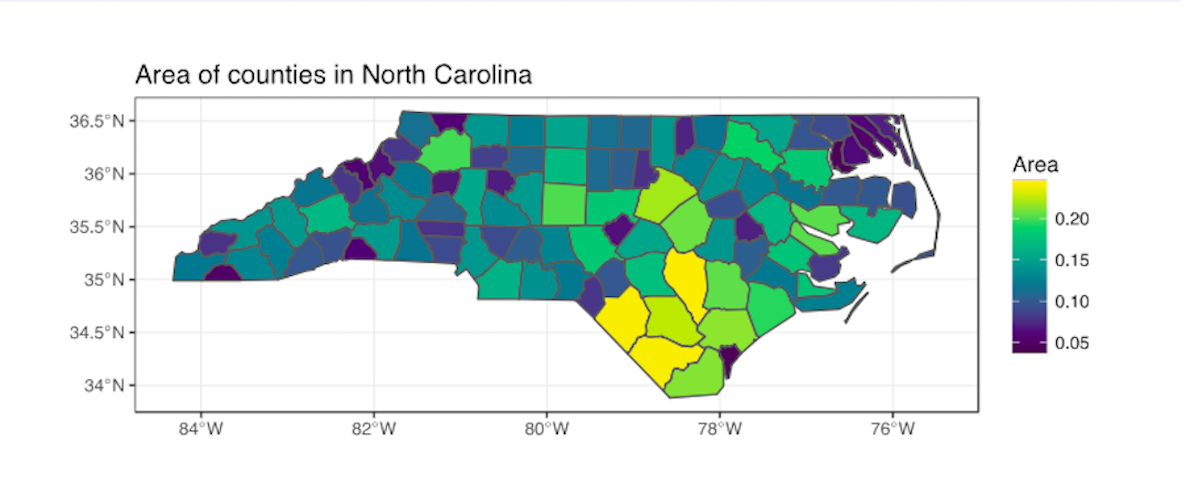
\includegraphics{sf.png}
\end{itemize}

\end{frame}

\hypertarget{r-basics}{%
\section{R Basics}\label{r-basics}}

\begin{frame}[fragile]{R as a calculator}
\protect\hypertarget{r-as-a-calculator}{}

\begin{Shaded}
\begin{Highlighting}[]
\DecValTok{5}
\CommentTok{#> [1] 5}
\DecValTok{5}\OperatorTok{+}\DecValTok{2}
\CommentTok{#> [1] 7}
\DecValTok{10}\OperatorTok{*}\DecValTok{3}
\CommentTok{#> [1] 30}
\end{Highlighting}
\end{Shaded}

\end{frame}

\begin{frame}[fragile]{Executing commands in R}
\protect\hypertarget{executing-commands-in-r}{}

\begin{Shaded}
\begin{Highlighting}[]
\DecValTok{5}
\CommentTok{#> [1] 5}
\DecValTok{5}\OperatorTok{+}\DecValTok{2}
\CommentTok{#> [1] 7}
\DecValTok{10}\OperatorTok{*}\DecValTok{3}
\CommentTok{#> [1] 30}
\end{Highlighting}
\end{Shaded}

Three ways to execute commands in R

\begin{enumerate}
\tightlist
\item
  Type/copy commands directly into the ``console''
\item
  `code chunks' in RMarkdown (.Rmd files)

  \begin{itemize}
  \tightlist
  \item
    Can execute one command at a time, one chunk at a time, or ``knit''
    the entire document
  \end{itemize}
\item
  R scripts (.R files)

  \begin{itemize}
  \tightlist
  \item
    This is just a text file full of R commands
  \item
    Can execute one command at a time, several commands at a time, or
    the entire script
  \end{itemize}
\end{enumerate}

\end{frame}

\begin{frame}[fragile]{Assignment}
\protect\hypertarget{assignment}{}

\textbf{Assignment} means creating a variable -- or more generally, an
``object'' -- and assigning values to it

\begin{itemize}
\tightlist
\item
  \texttt{\textless{}-} is the assignment operator

  \begin{itemize}
  \tightlist
  \item
    in other languages \texttt{=} is the assignment operator
  \end{itemize}
\item
  good practice to put a space before and after assignment operator
\end{itemize}

\begin{Shaded}
\begin{Highlighting}[]
\CommentTok{# Create an object and assign value}
\NormalTok{a <-}\StringTok{ }\DecValTok{5}
\NormalTok{a}
\CommentTok{#> [1] 5}

\NormalTok{b <-}\StringTok{ "yay!"}
\NormalTok{b}
\CommentTok{#> [1] "yay!"}
\end{Highlighting}
\end{Shaded}

\end{frame}

\hypertarget{directories-and-filepaths}{%
\section{Directories and filepaths}\label{directories-and-filepaths}}

\begin{frame}[fragile]{Working directory}
\protect\hypertarget{working-directory}{}

\textbf{(Current) Working directory}

\begin{itemize}
\tightlist
\item
  the folder/directory in which you are currently working
\item
  this is where R looks for files
\item
  Files located in your current working directory can be accessed
  without specifying a filepath because R automatically looks in this
  folder
\end{itemize}

Function \texttt{getwd()} shows current working directory

\begin{Shaded}
\begin{Highlighting}[]
\KeywordTok{getwd}\NormalTok{()}
\CommentTok{#> [1] "/Users/karinasalazar/Dropbox/HED612 Linear Regression/lectures/lecture1"}
\end{Highlighting}
\end{Shaded}

Command \texttt{list.files()} lists all files located in working
directory

\begin{Shaded}
\begin{Highlighting}[]
\KeywordTok{getwd}\NormalTok{()}
\CommentTok{#> [1] "/Users/karinasalazar/Dropbox/HED612 Linear Regression/lectures/lecture1"}
\KeywordTok{list.files}\NormalTok{()}
\CommentTok{#>  [1] "abor.png"                     "data-structures-overview.png"}
\CommentTok{#>  [3] "education.jpg"                "example1.html"               }
\CommentTok{#>  [5] "example1.Rmd"                 "HW1.pdf"                     }
\CommentTok{#>  [7] "HW1.Rmd"                      "lecture1_files"              }
\CommentTok{#>  [9] "lecture1.1_ua_files"          "lecture1.aux"                }
\CommentTok{#> [11] "lecture1.out"                 "lecture1.pdf"                }
\CommentTok{#> [13] "lecture1.Rmd"                 "lecture1.tex"                }
\CommentTok{#> [15] "lecture1.vrb"                 "normaldist.jpg"              }
\CommentTok{#> [17] "normaldist.png"               "pane_layout.png"             }
\CommentTok{#> [19] "professors.png"               "rticles.png"                 }
\CommentTok{#> [21] "sf.png"                       "shifts.jpg"                  }
\CommentTok{#> [23] "shifts.png"                   "shiny.png"                   }
\CommentTok{#> [25] "UpwardBoundLecture.pdf"       "UpwardBoundLecture.Rmd"      }
\CommentTok{#> [27] "UpwardBoundLecture.tex"       "women.png"}
\end{Highlighting}
\end{Shaded}

\end{frame}

\begin{frame}[fragile]{Absolute vs.~relative filepath}
\protect\hypertarget{absolute-vs.-relative-filepath}{}

\textbf{Absolute file path}: The absolute file path is the complete list
of directories needed to locate a file or folder.\\
\texttt{setwd("Users/Karina/rclass/lectures/lecture2")}

\textbf{Relative file path}: The relative file path is the path relative
to your current location/directory. Assuming your current working
directory is in the ``lecture2'' folder and you want to change your
directory to the data folder, your relative file path would look
something like this:\\
\texttt{setwd("../../data")}

\begin{verbatim}
        File path shortcuts
\end{verbatim}

\begin{longtable}[]{@{}ll@{}}
\toprule
\textbf{Key} & \textbf{Description}\tabularnewline
\midrule
\endhead
\textasciitilde{} & tilde is a shortcut for user's home directory (mine
is my name)\tabularnewline
../ & moves up a level\tabularnewline
../../ & moves up two level\tabularnewline
\bottomrule
\end{longtable}

\end{frame}

\hypertarget{create-r-project-and-directory-structure}{%
\section{Create ``R project'' and directory
structure}\label{create-r-project-and-directory-structure}}

\begin{frame}{What is an R project? Why are you doing this?}
\protect\hypertarget{what-is-an-r-project-why-are-you-doing-this}{}

What is an ``R project''?

\begin{itemize}
\tightlist
\item
  helps you keep all files for a project in one place
\item
  When you open an R project, the file-path of your current working
  directory is automatically set to the file-path of your R-project
\end{itemize}

Why am I asking you to create R project and download a specific
directory structure?

\begin{itemize}
\tightlist
\item
  I want you to be able to run the .R scripts for each lecture on your
  own computer
\item
  Sometimes these .R scripts point to certain sub-folders in order to
  open data
\item
  If you create the R project and create directory structure I
  recommend, you will be able to run .R scripts from your own computer
  without making any changes to file-paths!
\end{itemize}

\end{frame}

\begin{frame}{Follow these steps to create ``R project'' and directory
structure}
\protect\hypertarget{follow-these-steps-to-create-r-project-and-directory-structure}{}

\begin{enumerate}
\tightlist
\item
  Download the zip folder on D2L:

  \begin{itemize}
  \tightlist
  \item
    Unzip the folder: this is a shell of the file directory you should
    use for this class
  \item
    Move it to your preferred location (e.g, documents, desktop,
    dropbox, etc)
  \end{itemize}
\item
  In RStudio, click on ``File'' \textgreater\textgreater{} ``New
  Project'' \textgreater\textgreater{} ``New Directory''
  \textgreater\textgreater{} ``New Project''

  \begin{itemize}
  \tightlist
  \item
    In ``Directory name'', type ``hed612\_project'' as the title of the
    Rproject for the course
  \item
    In ``Create project as subdirectory of'', click browse and:

    \begin{itemize}
    \tightlist
    \item
      save the R Project within the hed612 folder (same general folder
      as data and lectures)
    \end{itemize}
  \end{itemize}
\end{enumerate}

\end{frame}

\begin{frame}{After you follow these steps}
\protect\hypertarget{after-you-follow-these-steps}{}

\begin{itemize}
\tightlist
\item
  You can add any additional sub-folders you want to the ``HED612''
  folder

  \begin{itemize}
  \tightlist
  \item
    e.g., ``syllabus'', ``homework''
  \end{itemize}
\item
  You can add any additional files you want to the sub-directory folders
  you unzipped

  \begin{itemize}
  \tightlist
  \item
    e.g., in ``HED612/lectures/lecture1'' you might add an additional
    document of notes you took
  \end{itemize}
\end{itemize}

\end{frame}

\hypertarget{next-week}{%
\section{Next Week}\label{next-week}}

\begin{frame}{Next Week}
\protect\hypertarget{next-week-1}{}

Next week will focus on reviewing intro statistics

\textbf{Reading}

\begin{itemize}
\tightlist
\item
  Heiss, pages 1-24 (stop at import/export of text files)
\item
  Stock \& Watson Chapter 3

  \begin{itemize}
  \tightlist
  \item
    Read/skim if you feel a bit rusty on some of the foundational
    concepts (t-tests, correlations, confidence intervals)
  \end{itemize}
\end{itemize}

\textbf{Problem Set \#1}

\begin{itemize}
\tightlist
\item
  Due next Wednesday 1/20/2021 at 4:15pm
\item
  Just giving you some practice with working within an R script and
  changing ``working directories'' via relative/absolute filepath
\end{itemize}

\end{frame}

\end{document}
